\documentclass[11pt,fleqn,a4paper]{book}

%%%%%%%%%%%%%%%%%%%%%%%%%%%%%%%%%%%%%%%%%
% The Legrand Orange Book
% Structural Definitions File
% Version 2.0 (9/2/15)
%
% Original author:
% Mathias Legrand (legrand.mathias@gmail.com) with modifications by:
% Vel (vel@latextemplates.com)
%
% This file has been downloaded from:
% http://www.LaTeXTemplates.com
%
% License:
% CC BY-NC-SA 3.0 (http://creativecommons.org/licenses/by-nc-sa/3.0/)
%
%%%%%%%%%%%%%%%%%%%%%%%%%%%%%%%%%%%%%%%%%

%----------------------------------------------------------------------------------------
%	VARIOUS REQUIRED PACKAGES AND CONFIGURATIONS
%----------------------------------------------------------------------------------------

\usepackage[top=3cm,bottom=3cm,left=3cm,right=3cm,headsep=10pt,a4paper]{geometry} % Page margins

\usepackage{graphicx} % Required for including pictures
\graphicspath{{img/}} % Specifies the directory where pictures are stored

\usepackage{titling} % Macros for title, author, etc
\usepackage{lipsum} % Inserts dummy text

\usepackage{tikz} % Required for drawing custom shapes

\usepackage[english,dutch]{babel} % English language/hyphenation
\usepackage{iflang}

\usepackage{enumitem} % Customize lists
\setlist{nolistsep} % Reduce spacing between bullet points and numbered lists

\usepackage{booktabs} % Required for nicer horizontal rules in tables

\usepackage{xcolor} % Required for specifying colors by name
\definecolor{maincolor}{RGB}{0,100,184} % Define the main color used for highlighting throughout the book

% Paragraph style: no indent, add space between paragraphs
\setlength{\parindent}{0em}
\setlength{\parskip}{1em}

%----------------------------------------------------------------------------------------
%	FONTS
%----------------------------------------------------------------------------------------

\usepackage{avant} % Use the Avantgarde font for headings
%\usepackage{times} % Use the Times font for headings
\usepackage{mathptmx} % Use the Adobe Times Roman as the default text font together with math symbols from the Sym­bol, Chancery and Com­puter Modern fonts
\usepackage{eurosym}

\usepackage{amsfonts}
\usepackage{amsmath}
\usepackage{amssymb}
\usepackage{textcomp}
\usepackage{wasysym}

\usepackage{microtype} % Slightly tweak font spacing for aesthetics
\usepackage[utf8]{inputenc} % Required for including letters with accents
\usepackage[T1]{fontenc} % Use 8-bit encoding that has 256 glyphs

%------------------------------------------------------------------------------
%	TITLE PAGE
%------------------------------------------------------------------------------

\newcommand{\thetitlepage}{%
\begingroup
\thispagestyle{empty}
\begin{tikzpicture}[remember picture,overlay]
\coordinate [below=12cm] (midpoint) at (current page.north);
\node at (current page.north west)
{\begin{tikzpicture}[remember picture,overlay]
\node[anchor=north west,inner sep=0pt] at (0,0) {
\includegraphics[width=\paperwidth]{background}}; % Background image
\draw[anchor=north] (midpoint) node [fill=maincolor,fill opacity=0,text=white,text opacity=1,inner sep=1cm]{\Huge\centering\bfseries\sffamily\parbox[c][][t]{\paperwidth}{\centering \thetitle\\[15pt] % Book title
{\Large \thedate}\\[20pt] % Subtitle
{\large \theauthor}}}; % Author name
\end{tikzpicture}};
\end{tikzpicture}
\vfill
\endgroup
}

%----------------------------------------------------------------------------------------
%	BIBLIOGRAPHY AND INDEX
%----------------------------------------------------------------------------------------

\usepackage[style=apa,backend=biber]{biblatex}
\usepackage{csquotes}
\DeclareLanguageMapping{dutch}{dutch-apa}
\addbibresource{bibliografie.bib} % BibTeX bibliography file
\defbibheading{bibempty}{}

\usepackage{calc} % For simpler calculation - used for spacing the index letter headings correctly
\usepackage{makeidx} % Required to make an index
\makeindex % Tells LaTeX to create the files required for indexing

%----------------------------------------------------------------------------------------
%	MAIN TABLE OF CONTENTS
%----------------------------------------------------------------------------------------

\usepackage{titletoc} % Required for manipulating the table of contents

\contentsmargin{0cm} % Removes the default margin

% Part text styling
\titlecontents{part}[0cm]
{\addvspace{20pt}\centering\large\bfseries}
{}
{}
{}

% Chapter text styling
\titlecontents{chapter}[1.25cm] % Indentation
{\addvspace{12pt}\large\sffamily\bfseries} % Spacing and font options for chapters
{\color{maincolor!60}\contentslabel[\Large\thecontentslabel]{1.25cm}\color{maincolor}} % Chapter number
{\color{maincolor}}
{\color{maincolor!60}\normalsize\;\titlerule*[.5pc]{.}\;\thecontentspage} % Page number

% Section text styling
\titlecontents{section}[1.25cm] % Indentation
{\addvspace{3pt}\sffamily\bfseries} % Spacing and font options for sections
{\contentslabel[\thecontentslabel]{1.25cm}} % Section number
{}
{\hfill\color{black}\thecontentspage} % Page number
[]

% Subsection text styling
\titlecontents{subsection}[1.25cm] % Indentation
{\addvspace{1pt}\sffamily\small} % Spacing and font options for subsections
{\contentslabel[\thecontentslabel]{1.25cm}} % Subsection number
{}
{\ \titlerule*[.5pc]{.}\;\thecontentspage} % Page number
[]

% List of figures
\titlecontents{figure}[0em]
{\addvspace{-5pt}\sffamily}
{\thecontentslabel\hspace*{1em}}
{}
{\ \titlerule*[.5pc]{.}\;\thecontentspage}
[]

% List of tables
\titlecontents{table}[0em]
{\addvspace{-5pt}\sffamily}
{\thecontentslabel\hspace*{1em}}
{}
{\ \titlerule*[.5pc]{.}\;\thecontentspage}
[]

%----------------------------------------------------------------------------------------
%	MINI TABLE OF CONTENTS IN PART HEADS
%----------------------------------------------------------------------------------------

% Chapter text styling
\titlecontents{lchapter}[0em] % Indenting
{\addvspace{15pt}\large\sffamily\bfseries} % Spacing and font options for chapters
{\color{maincolor}\contentslabel[\Large\thecontentslabel]{1.25cm}\color{maincolor}} % Chapter number
{}
{\color{maincolor}\normalsize\sffamily\bfseries\;\titlerule*[.5pc]{.}\;\thecontentspage} % Page number

% Section text styling
\titlecontents{lsection}[0em] % Indenting
{\sffamily\small} % Spacing and font options for sections
{\contentslabel[\thecontentslabel]{1.25cm}} % Section number
{}
{}

% Subsection text styling
\titlecontents{lsubsection}[.5em] % Indentation
{\normalfont\footnotesize\sffamily} % Font settings
{}
{}
{}

%----------------------------------------------------------------------------------------
%	PAGE HEADERS
%----------------------------------------------------------------------------------------

\usepackage{fancyhdr} % Required for header and footer configuration

\pagestyle{fancy}
\renewcommand{\chaptermark}[1]{\markboth{\sffamily\normalsize\bfseries\chaptername\ \thechapter.\ #1}{}} % Chapter text font settings
\renewcommand{\sectionmark}[1]{\markright{\sffamily\normalsize\thesection\hspace{5pt}#1}{}} % Section text font settings
\fancyhf{} \fancyhead[LE,RO]{\sffamily\normalsize\thepage} % Font setting for the page number in the header
\fancyhead[LO]{\rightmark} % Print the nearest section name on the left side of odd pages
\fancyhead[RE]{\leftmark} % Print the current chapter name on the right side of even pages
\renewcommand{\headrulewidth}{0.5pt} % Width of the rule under the header
\addtolength{\headheight}{2.5pt} % Increase the spacing around the header slightly
\renewcommand{\footrulewidth}{0pt} % Removes the rule in the footer
\fancypagestyle{plain}{\fancyhead{}\renewcommand{\headrulewidth}{0pt}} % Style for when a plain pagestyle is specified

% Removes the header from odd empty pages at the end of chapters
\makeatletter
\renewcommand{\cleardoublepage}{
\clearpage\ifodd\c@page\else
\hbox{}
\vspace*{\fill}
\thispagestyle{empty}
\newpage
\fi}

%----------------------------------------------------------------------------------------
%	THEOREM STYLES
%----------------------------------------------------------------------------------------

\usepackage{amsmath,amsfonts,amssymb,amsthm} % For math equations, theorems, symbols, etc

\newcommand{\intoo}[2]{\mathopen{]}#1\,;#2\mathclose{[}}
\newcommand{\ud}{\mathop{\mathrm{{}d}}\mathopen{}}
\newcommand{\intff}[2]{\mathopen{[}#1\,;#2\mathclose{]}}
\newtheorem{notation}{Notation}[chapter]

% Boxed/framed environments
\newtheoremstyle{maincolornumbox}% % Theorem style name
{0pt}% Space above
{0pt}% Space below
{\normalfont}% % Body font
{}% Indent amount
{\small\bf\sffamily\color{maincolor}}% % Theorem head font
{\;}% Punctuation after theorem head
{0.25em}% Space after theorem head
{\small\sffamily\color{maincolor}\thmname{#1}\nobreakspace\thmnumber{\@ifnotempty{#1}{}\@upn{#2}}% Theorem text (e.g. Theorem 2.1)
\thmnote{\nobreakspace\the\thm@notefont\sffamily\bfseries\color{black}---\nobreakspace#3.}} % Optional theorem note
\renewcommand{\qedsymbol}{$\blacksquare$}% Optional qed square

\newtheoremstyle{blacknumex}% Theorem style name
{5pt}% Space above
{5pt}% Space below
{\normalfont}% Body font
{} % Indent amount
{\small\bf\sffamily}% Theorem head font
{\;}% Punctuation after theorem head
{0.25em}% Space after theorem head
{\small\sffamily{\tiny\ensuremath{\blacksquare}}\nobreakspace\thmname{#1}\nobreakspace\thmnumber{\@ifnotempty{#1}{}\@upn{#2}}% Theorem text (e.g. Theorem 2.1)
\thmnote{\nobreakspace\the\thm@notefont\sffamily\bfseries---\nobreakspace#3.}}% Optional theorem note

\newtheoremstyle{blacknumbox} % Theorem style name
{0pt}% Space above
{0pt}% Space below
{\normalfont}% Body font
{}% Indent amount
{\small\bf\sffamily}% Theorem head font
{\;}% Punctuation after theorem head
{0.25em}% Space after theorem head
{\small\sffamily\thmname{#1}\nobreakspace\thmnumber{\@ifnotempty{#1}{}\@upn{#2}}% Theorem text (e.g. Theorem 2.1)
\thmnote{\nobreakspace\the\thm@notefont\sffamily\bfseries---\nobreakspace#3.}}% Optional theorem note

% Non-boxed/non-framed environments
\newtheoremstyle{maincolornum}% % Theorem style name
{5pt}% Space above
{5pt}% Space below
{\normalfont}% % Body font
{}% Indent amount
{\small\bf\sffamily\color{maincolor}}% % Theorem head font
{\;}% Punctuation after theorem head
{0.25em}% Space after theorem head
{\small\sffamily\color{maincolor}\thmname{#1}\nobreakspace\thmnumber{\@ifnotempty{#1}{}\@upn{#2}}% Theorem text (e.g. Theorem 2.1)
\thmnote{\nobreakspace\the\thm@notefont\sffamily\bfseries\color{black}---\nobreakspace#3.}} % Optional theorem note
\renewcommand{\qedsymbol}{$\blacksquare$}% Optional qed square
\makeatother

% Defines the theorem text style for each type of theorem to one of the three styles above
\newcounter{dummy}
\numberwithin{dummy}{section}
\theoremstyle{maincolornumbox}
\newtheorem{theoremeT}[dummy]{Theorem}
\newtheorem{problem}{Problem}[chapter]
\newtheorem{exerciseT}{Exercise}[chapter]
\theoremstyle{blacknumex}
\newtheorem{exampleT}{Example}[chapter]
\theoremstyle{blacknumbox}
\newtheorem{vocabulary}{Vocabulary}[chapter]
\newtheorem{definitionT}{Definition}[section]
\newtheorem{corollaryT}[dummy]{Corollary}
\theoremstyle{maincolornum}
\newtheorem{proposition}[dummy]{Proposition}

%----------------------------------------------------------------------------------------
%	DEFINITION OF COLORED BOXES
%----------------------------------------------------------------------------------------

\RequirePackage[framemethod=default]{mdframed} % Required for creating the theorem, definition, exercise and corollary boxes

% Theorem box
\newmdenv[skipabove=7pt,
skipbelow=7pt,
backgroundcolor=black!5,
linecolor=maincolor,
innerleftmargin=5pt,
innerrightmargin=5pt,
innertopmargin=5pt,
leftmargin=0cm,
rightmargin=0cm,
innerbottommargin=5pt]{tBox}

% Exercise box
\newmdenv[skipabove=7pt,
skipbelow=7pt,
rightline=false,
leftline=true,
topline=false,
bottomline=false,
backgroundcolor=maincolor!10,
linecolor=maincolor,
innerleftmargin=5pt,
innerrightmargin=5pt,
innertopmargin=5pt,
innerbottommargin=5pt,
leftmargin=0cm,
rightmargin=0cm,
linewidth=4pt]{eBox}

% Definition box
\newmdenv[skipabove=7pt,
skipbelow=7pt,
rightline=false,
leftline=true,
topline=false,
bottomline=false,
linecolor=maincolor,
innerleftmargin=5pt,
innerrightmargin=5pt,
innertopmargin=0pt,
leftmargin=0cm,
rightmargin=0cm,
linewidth=4pt,
innerbottommargin=0pt]{dBox}

% Corollary box
\newmdenv[skipabove=7pt,
skipbelow=7pt,
rightline=false,
leftline=true,
topline=false,
bottomline=false,
linecolor=gray,
backgroundcolor=black!5,
innerleftmargin=5pt,
innerrightmargin=5pt,
innertopmargin=5pt,
leftmargin=0cm,
rightmargin=0cm,
linewidth=4pt,
innerbottommargin=5pt]{cBox}

% Creates an environment for each type of theorem and assigns it a theorem text style from the "Theorem Styles" section above and a colored box from above
\newenvironment{theorem}{\begin{tBox}\begin{theoremeT}}{\end{theoremeT}\end{tBox}}
\newenvironment{exercise}{\begin{eBox}\begin{exerciseT}}{\hfill{\color{maincolor}\tiny\ensuremath{\blacksquare}}\end{exerciseT}\end{eBox}}
\newenvironment{definition}{\begin{dBox}\begin{definitionT}}{\end{definitionT}\end{dBox}}
\newenvironment{example}{\begin{exampleT}}{\hfill{\tiny\ensuremath{\blacksquare}}\end{exampleT}}
\newenvironment{corollary}{\begin{cBox}\begin{corollaryT}}{\end{corollaryT}\end{cBox}}

%----------------------------------------------------------------------------------------
%	REMARK ENVIRONMENT
%----------------------------------------------------------------------------------------

\newenvironment{remark}{\par\vspace{10pt}\small % Vertical white space above the remark and smaller font size
\begin{list}{}{
\leftmargin=35pt % Indentation on the left
\rightmargin=25pt}\item\ignorespaces % Indentation on the right
\makebox[-2.5pt]{\begin{tikzpicture}[overlay]
\node[draw=maincolor!60,line width=1pt,circle,fill=maincolor!25,font=\sffamily\bfseries,inner sep=2pt,outer sep=0pt] at (-15pt,0pt){\textcolor{maincolor}{R}};\end{tikzpicture}} % Orange R in a circle
\advance\baselineskip -1pt}{\end{list}\vskip5pt} % Tighter line spacing and white space after remark

%----------------------------------------------------------------------------------------
%	SECTION NUMBERING IN THE MARGIN
%----------------------------------------------------------------------------------------

\makeatletter
\renewcommand{\@seccntformat}[1]{\llap{\textcolor{maincolor}{\csname the#1\endcsname}\hspace{1em}}}
\renewcommand{\section}{\@startsection{section}{1}{\z@}
{-4ex \@plus -1ex \@minus -.4ex}
{1ex \@plus.2ex }
{\normalfont\large\sffamily\bfseries}}
\renewcommand{\subsection}{\@startsection {subsection}{2}{\z@}
{-3ex \@plus -0.1ex \@minus -.4ex}
{0.5ex \@plus.2ex }
{\normalfont\sffamily\bfseries}}
\renewcommand{\subsubsection}{\@startsection {subsubsection}{3}{\z@}
{-2ex \@plus -0.1ex \@minus -.2ex}
{.2ex \@plus.2ex }
{\normalfont\small\sffamily\bfseries}}
\renewcommand\paragraph{\@startsection{paragraph}{4}{\z@}
{-2ex \@plus-.2ex \@minus .2ex}
{.1ex}
{\normalfont\small\sffamily\bfseries}}

%----------------------------------------------------------------------------------------
%	PART HEADINGS
%----------------------------------------------------------------------------------------

% numbered part in the table of contents
\newcommand{\@mypartnumtocformat}[2]{%
\setlength\fboxsep{0pt}%
\noindent\colorbox{maincolor!20}{\strut\parbox[c][.7cm]{\ecart}{\color{maincolor!70}\Large\sffamily\bfseries\centering#1}}\hskip\esp\colorbox{maincolor!40}{\strut\parbox[c][.7cm]{\linewidth-\ecart-\esp}{\Large\sffamily\centering#2}}}%
%%%%%%%%%%%%%%%%%%%%%%%%%%%%%%%%%%
% unnumbered part in the table of contents
\newcommand{\@myparttocformat}[1]{%
\setlength\fboxsep{0pt}%
\noindent\colorbox{maincolor!40}{\strut\parbox[c][.7cm]{\linewidth}{\Large\sffamily\centering#1}}}%
%%%%%%%%%%%%%%%%%%%%%%%%%%%%%%%%%%
\newlength\esp
\setlength\esp{4pt}
\newlength\ecart
\setlength\ecart{1.2cm-\esp}
\newcommand{\thepartimage}{}%
\newcommand{\partimage}[1]{\renewcommand{\thepartimage}{#1}}%
\def\@part[#1]#2{%
\ifnum \c@secnumdepth >-2\relax%
\refstepcounter{part}%
\addcontentsline{toc}{part}{\texorpdfstring{\protect\@mypartnumtocformat{\thepart}{#1}}{\partname~\thepart\ ---\ #1}}
\else%
\addcontentsline{toc}{part}{\texorpdfstring{\protect\@myparttocformat{#1}}{#1}}%
\fi%
\startcontents%
\markboth{}{}%
{\thispagestyle{empty}%
\begin{tikzpicture}[remember picture,overlay]%
\node at (current page.north west){\begin{tikzpicture}[remember picture,overlay]%
\fill[maincolor!20](0cm,0cm) rectangle (\paperwidth,-\paperheight);
\node[anchor=north] at (4cm,-3.25cm){\color{maincolor!40}\fontsize{220}{100}\sffamily\bfseries\@Roman\c@part};
\node[anchor=south east] at (\paperwidth-1cm,-\paperheight+1cm){\parbox[t][][t]{8.5cm}{
\printcontents{l}{0}{\setcounter{tocdepth}{1}}%
}};
\node[anchor=north east] at (\paperwidth-1.5cm,-3.25cm){\parbox[t][][t]{15cm}{\strut\raggedleft\color{white}\fontsize{30}{30}\sffamily\bfseries#2}};
\end{tikzpicture}};
\end{tikzpicture}}%
\@endpart}
\def\@spart#1{%
\startcontents%
\phantomsection
{\thispagestyle{empty}%
\begin{tikzpicture}[remember picture,overlay]%
\node at (current page.north west){\begin{tikzpicture}[remember picture,overlay]%
\fill[maincolor!20](0cm,0cm) rectangle (\paperwidth,-\paperheight);
\node[anchor=north east] at (\paperwidth-1.5cm,-3.25cm){\parbox[t][][t]{15cm}{\strut\raggedleft\color{white}\fontsize{30}{30}\sffamily\bfseries#1}};
\end{tikzpicture}};
\end{tikzpicture}}
\addcontentsline{toc}{part}{\texorpdfstring{%
\setlength\fboxsep{0pt}%
\noindent\protect\colorbox{maincolor!40}{\strut\protect\parbox[c][.7cm]{\linewidth}{\Large\sffamily\protect\centering #1\quad\mbox{}}}}{#1}}%
\@endpart}
\def\@endpart{\vfil\newpage
\if@twoside
\if@openright
\null
\thispagestyle{empty}%
\newpage
\fi
\fi
\if@tempswa
\twocolumn
\fi}

%----------------------------------------------------------------------------------------
%	CHAPTER HEADINGS
%----------------------------------------------------------------------------------------

% A switch to conditionally include a picture, implemented by  Christian Hupfer
\newif\ifusechapterimage
\usechapterimagetrue
\newcommand{\thechapterimage}{}%
\newcommand{\chapterimage}[1]{\ifusechapterimage\renewcommand{\thechapterimage}{#1}\fi}%
\def\@makechapterhead#1{%
{\parindent \z@ \raggedright \normalfont
\ifnum \c@secnumdepth >\m@ne
\if@mainmatter
\begin{tikzpicture}[remember picture,overlay]
\node at (current page.north west)
{\begin{tikzpicture}[remember picture,overlay]
\node[anchor=north west,inner sep=0pt] at (0,0) {\ifusechapterimage\includegraphics[width=\paperwidth]{\thechapterimage}\fi};
\draw[anchor=west] (\Gm@lmargin,-9cm) node [line width=2pt,rounded corners=15pt,draw=maincolor,fill=white,fill opacity=0.5,inner sep=15pt]{\strut\makebox[22cm]{}};
\draw[anchor=west] (\Gm@lmargin+.3cm,-9cm) node {\huge\sffamily\bfseries\color{black}\thechapter. #1\strut};
\end{tikzpicture}};
\end{tikzpicture}
\else
\begin{tikzpicture}[remember picture,overlay]
\node at (current page.north west)
{\begin{tikzpicture}[remember picture,overlay]
\node[anchor=north west,inner sep=0pt] at (0,0) {\ifusechapterimage\includegraphics[width=\paperwidth]{\thechapterimage}\fi};
\draw[anchor=west] (\Gm@lmargin,-9cm) node [line width=2pt,rounded corners=15pt,draw=maincolor,fill=white,fill opacity=0.5,inner sep=15pt]{\strut\makebox[22cm]{}};
\draw[anchor=west] (\Gm@lmargin+.3cm,-9cm) node {\huge\sffamily\bfseries\color{black}#1\strut};
\end{tikzpicture}};
\end{tikzpicture}
\fi\fi\par\vspace*{270\p@}}}

%-------------------------------------------

\def\@makeschapterhead#1{%
\begin{tikzpicture}[remember picture,overlay]
\node at (current page.north west)
{\begin{tikzpicture}[remember picture,overlay]
\node[anchor=north west,inner sep=0pt] at (0,0) {\ifusechapterimage\includegraphics[width=\paperwidth]{\thechapterimage}\fi};
\draw[anchor=west] (\Gm@lmargin,-9cm) node [line width=2pt,rounded corners=15pt,draw=maincolor,fill=white,fill opacity=0.5,inner sep=15pt]{\strut\makebox[22cm]{}};
\draw[anchor=west] (\Gm@lmargin+.3cm,-9cm) node {\huge\sffamily\bfseries\color{black}#1\strut};
\end{tikzpicture}};
\end{tikzpicture}
\par\vspace*{270\p@}}
\makeatother

%----------------------------------------------------------------------------------------
%	HYPERLINKS IN THE DOCUMENTS
%----------------------------------------------------------------------------------------

\usepackage{hyperref}
\hypersetup{hidelinks,backref=true,pagebackref=true,hyperindex=true,colorlinks=false,breaklinks=true,urlcolor= maincolor,bookmarks=true,bookmarksopen=false,pdftitle={Title},pdfauthor={Author}}
\usepackage{bookmark}
\bookmarksetup{
open,
numbered,
addtohook={%
\ifnum\bookmarkget{level}=0 % chapter
\bookmarksetup{bold}%
\fi
\ifnum\bookmarkget{level}=-1 % part
\bookmarksetup{color=maincolor,bold}%
\fi
}
}


\newcommand{\acadj}{2016-2017}

\author{Bert Van Vreckem}
\title{Syllabus Enterprise Linux}
\date{Academiejaar \acadj}

\begin{document}

\thetitlepage

%---------- Colofon -----------------------------------------------------------

\newpage
~\vfill
\thispagestyle{empty}

\noindent Copyright \copyright\ 2016 Bert Van Vreckem\\ % Copyright notice

\noindent \textit{Dit werk valt onder de \href{http://creativecommons.org/licenses/by-sa/4.0/}{Creative Commons Naamsvermelding-GelijkDelen 4.0 Internationale Publieke Licentie}. De vormgeving is gebaseerd op ``\href{http://www.latextemplates.com/template/the-legrand-orange-book}{The Legrand Orange Book}'' door Mathias Legrand}\\

\noindent \textit{\today} % Printing/edition date

%---------- Inhoudstafel ------------------------------------------------------
\usechapterimagefalse

\tableofcontents % Print the table of contents itself

\cleardoublepage % Forces the first chapter to start on an odd page so it's on the right

%---------- Corpus ------------------------------------------------------------
\chapter{Cursusorganisatie}
\label{cursusorganisatie}

\section{Praktische afspraken}
\label{praktische-afspraken}

Wat betreft praktische afspraken, regelingen, verwachtingen, enz. in
verband met deze cursus zijn dit de enige geldige bronnen van
informatie:

\begin{itemize}
\item
  De
  \href{https://bamaflexweb.hogent.be/BMFUIDetailxOLOD.aspx?a=68521\&b=5\&c=1}{ECTS-fiche}
  van het opleidingsonderdeel
\item
  Deze studiewijzer
\item
  Aankondigingen en documenten op Chamilo
\end{itemize}

Indien er ergens twijfel over bestaat, of er is iets niet duidelijk,
neem dan zo snel mogelijk contact op met de vaktitularis
(\href{mailto:bert.vanvreckem@hogent.be}{Bert Van Vreckem}), hetzij
tijdens de contactmomenten, hetzij via e-mail. Indien nuttig of nodig
wordt het antwoord als aankondiging op Chamilo doorgegeven aan alle
studenten. De ervaring leert dat de onderlinge communicatie tussen
studenten via Facebook leidt tot verwarring, foute informatie en
discussie achteraf. Gebruik dus aub de officiële kanalen zodat we tot
een open en correcte communicatie rond deze cursus kunnen komen.

Jullie zijn zelf verantwoordelijk voor het opvolgen en lezen van alle
aankondigingen.

\section{Opzet lessen}
\label{opzet-lessen}

In deze cursus zijn er \textbf{geen theorielessen}. Bij aanvang van het
semester krijg je een uitleg over het opzet van de cursus en over
praktische afspraken, maar in principe is dat de enige keer dat er een
plenaire uitleg komt. Er worden tal van (vrij beschikbare) studiematerialen aangereikt die je in staat moeten stellen de nodige achtergrondinformatie zelf te verwerken.

De lectoren van de leerlijn systeem- en netwerkbeheer zijn de
mening toegedaan dat ons vakdomein er één is dat je enkel kan eigen
maken door \textbf{praktijkervaring} op te doen. Bovendien evolueert het
vakgebied zo snel dat bijleren en informatie over nieuwe
technologieën of tools opzoeken en verwerken een vast onderdeel is van de job.

Tijdens de contactmomenten willen we daarom maximaal tijd vrij maken om
met de praktijk bezig te zijn aan de hand van labo-taken. Dat vereist
een zekere mate van zelfstandigheid, maar dat is precies ook een
attitude die verwacht wordt van een systeembeheerder. Je neemt dus zelf
initiatief om de nodige kennis te vergaren en zoekt naar oplossingen
voor de problemen die je ongetwijfeld zal tegenkomen. Help elkaar
daarin: samenwerken en kennis delen wordt van harte aangemoedigd. De
lector is uiteraard ook beschikbaar om je bij te staan als je toch vast
komt te zitten en kan je tips geven of verwijzen naar geschikte
studiematerialen.

\section{Evaluatie}
\label{evaluatie}

De evaluatie van dit vak is volledig op basis van niet-periodegebonden
evaluatie. Je wordt beoordeeld op de volgende opdrachten:

\begin{itemize}
\item
  Labo-opdracht opzetten infrastructuur met een configuration management
  system
\item
  Taak rond actualiteit in het vakgebied
\item
  Troubleshooting van netwerkservices
\item
  Rapportering en documentatie
\end{itemize}

Verderop wordt in meer detail uitgelegd wat precies verwacht wordt. De
toekenning van het examencijfer gebeurt op basis van ``rubrics''~\autocite{Andrade2000}. In een
tabel worden een aantal criteria opgesomd, waar je aan moet voldoen. Je
kan ``voldoen'' op verschillende niveaus, meer bepaald ``bekwaam'',
``gevorderd'', ``deskundig'', of in het slechtste geval ``nog niet
bekwaam''. Voor elk niveau wordt beschreven wat dat precies inhoudt. Het
volledige evaluatieschema wordt tijdig op Chamilo gepubliceerd.

Om te slagen voor dit vak moet je aantonen dat je voor \textbf{alle} technische
criteria minstens ``bekwaam'' bent. Met andere woorden, wie voor één
criterium ``nog niet bekwaam'' bevonden wordt, kan niet slagen. De
niet-technische criteria (bv. rapportering) wegen minder zwaar mee, maar
als je hier ``nog niet bekwaam'' bevonden wordt, zal dit het
examencijfer negatief beïnvloeden.

Je bekwaamheid aantonen gebeurt aan de hand van volgende deliverables:

\begin{itemize}
\item
  De broncode, door elke student bijgehouden in een toegewezen Git
  repository
\item
  Gedetailleerde labo-verslagen, eveneens bijgehouden in Git
\item
  Demonstratie van deelresultaten aan de lector tijdens het semester
\item
  Demonstratie van het eindresultaat aan de lector tijdens de
  examenperiode
\end{itemize}

\textbf{Merk op} dat je zowel een werkend product moet opleveren (= broncode) als de verslagen indienen én demo's geven. Als één van de deliverables ontbreekt, wordt de opdracht beschouwd als niet gerealiseerd. Je moet minstens elke drie weken deelresulaten opleveren en persoonlijk demonstreren aan de lector (voor studenten TILE: zie verder).

Wat betreft het respecteren van deadlines is art. 34 van het FOER van kracht. Niet tijdig deelresultaten demonstreren wordt in termen van dat artikel beschouwd als het niet respecteren van tussentijdse deadlines en wordt als dusdanig gesanctioneerd. Eén van de opdrachten (zoals hierboven opgesomd) niet realiseren leidt tot een afwezigheid voor die opdracht en bijgevolg ook voor het gehele opleidingsonderdeel, conform het examenreglement.

\subsection{Afstandsleren (TILE)}
\label{afstandsleren-tile}

Wie de cursus volgt via afstandsleren voert dezelfde opdrachten uit en
wordt op dezelfde manier geëvalueerd. Dat betekent ook dat je regelmatig
deelresultaten demonstreert aan de lector. Dat kan op verschillende
manieren:

\begin{itemize}
\item aan de hand van een screencast (bv. publiceren op Youtube, link doorsturen naar de lector),
\item via videoconferencing (Google Hangouts of Skype, na afspraak),
\item tijdens de contactmomenten voor TILE-studenten, als de lector daar aanwezig is (en enkel na afspraak),
\item tijdens de normale contactmomenten, zowel op campus Aalst (dinsdag 9:15 - 12:30, lokaal GAARB.0.029) als Gent (woensdag 9:15 - 12:30, lokaal B4.037).
\end{itemize}

Voor de troubleshooting-oefeningen (zie verder) kan je met de lector een moment afspreken waarop je tijd hebt om hier aan te werken. Op het afgesproken tijdstip krijg je een downloadlink naar de opgave en dien je voor de afgesproken deadline (in principe 3 uur na ontvangst van de opgave) in op Chamilo.

Vragen kan je stellen per e-mail of op de contactmomenten voor TILE.

\subsection{Tweede examenkans}
\label{tweede-examenkans}

Wie niet slaagt dient voor de tweede zittijd een individuele opdracht uit te voeren. De precieze opdracht hangt af van je evaluatie. Meer bepaald zal je moet kunnen aantonen dat je voor alle technische criteria minstens ``bekwaam'' bent. Deze opdracht wordt vastgelegd op de feedback.

\textbf{Wie vóór het ingaan van het intersemestrieel reces geen afspraken maakt ivm een individuele opdracht, geeft daarmee te kennen niet te willen deelnemen aan de tweede zittijd.}

\section{Gebruikte hard- en software}
\label{gebruikte-hard--en-software}

De aard van deze cursus maakt dat het essentieel is dat je beschikt over voldoende krachtige hardware. Op campus Schoonmeersen kan je gebruik maken van de klaspc's, maar blijft het belangrijk om ook thuis of op kot te kunnen verder werken. Enkele aanbevelingen:

\begin{itemize}
\item Processor: Intel i7 of equivalent (een i5 is voldoende, maar wie een i3-processor heeft wordt sterk aangeraden te investeren)
\item Geheugen: 8 GiB RAM
\item Harde schijf: 40 GB vrije schijfruimte is ruim voldoende
\end{itemize}

Voor het uitwerken van de labo-taken maak je gebruik van de hieronder opgesomde software (in principe de laatste stabiele versies bij aanvang van het semester). Als je sommige van de opgesomde applicaties al geïnstalleerd hebt, werk die dan bij tot de laatste versie.

\begin{itemize}
\item Een \textbf{degelijke} teksteditor: Sublime, Notepad++, Vim, enz.
  \begin{itemize}
  \item Let op! Stel je editor zo in dat tekst inspringt met \textbf{spaties} i.p.v. tabs en zet tabbreedte op 2 karakters.
  \end{itemize}
\item VirtualBox 5.x\footnote{\url{https://www.virtualbox.org/wiki/Downloads}} (installeer ook het ``Extension Pack'').
\item Vagrant\footnote{\url{http://vagrantup.com/}} \textgreater{}= 1.8.4
\item Git\footnote{\url{https://git-scm.com/downloads}}
\item Bash shell. Onder Windows, kan je de Bash shell die meegeleverd wordt met Git gebruiken. Mac gebruikers wordt aangeraden om een recente versie van Bash te installeren, bijvoorbeeld via HomeBrew.
\item Ansible\footnote{\url{https://docs.ansible.com/ansible/intro_installation.html}} \textgreater{}= 2.1 (enkel voor wie werkt met een Mac of Linux-laptop, Windows-gebruikers kunnen dit niet installeren maar voor hen is een workaround voorzien)
\item Optioneel:

  \begin{itemize}
    \item Een teksteditor voor Markdown\footnote{\url{http://daringfireball.net/projects/markdown/}}, bijvoorbeeld MarkdownPad\footnote{\url{http://markdownpad.com/}}, Texts\footnote{\url{http://www.texts.io/}}, enz.
  \item Pandoc\footnote{\url{http://johnmacfarlane.net/pandoc/}} en \LaTeX\ voor het
    omzetten van documentatie in Markdown naar PDF.
  \end{itemize}
\end{itemize}

Verder komt het volgende nog van pas:

\begin{itemize}
\item Een USB-stick of externe USB-schijf met voldoende ruimte (voor het bijhouden van VMs en broncode)
\item Een netwerkkabel en RJ-45 koppelstuk (netwerklokaal c.Schoonmeersen)
\item Oortjes voor het beluisteren/bekijken van videolessen, screencasts of videopresentaties zonder de rest te storen
\end{itemize}

\section{Wat moet je kennen en kunnen?}
\label{wat-moet-je-kennen-en-kunnen}

\subsection{Leerdoelen}
\label{leerdoelen}

De belangrijkste doelstellingen van deze cursus (die je ook vindt in de studiefiche\footnote{\url{https://bamaflexweb.hogent.be/BMFUIDetailxOLOD.aspx?a=77579&b=5&c=1}}) zijn:

\begin{itemize}
\item Netwerkservices kunnen opzetten in Linux, voor middelgrote tot grote ondernemingen (wat een bijzondere nadruk op automatisering impliceert);
\item Systematisch en grondig troubleshooten;
\item De meest relevante informatie kunnen opzoeken specifiek voor het systeem waar je mee werkt.
\end{itemize}

\subsection{Te bekijken videolessen, -tutorials, enz.}
\label{te-bekijken-videolessen--tutorials-enz.}

% TODO: is dit de beste plaats hiervoor?

\begin{itemize}
  \item SELinux for mere mortals~\autocite{Cameron2012}
  \item Ansible: Python-Powered Radically Simple IT Automation~\autocite{DeHaan2014}
  \item Vijf trends in systeembeheer, inleidingsles Enterprise Linux~\autocite{VanVreckem2013}
\end{itemize}

\subsection{Documentatie gebruiken}
\label{documentatie-gebruiken}

Je moet in staat zijn de juiste documentatie op te zoeken en te gebruiken, die relevant is voor het systeem waar je mee werkt, i.h.b. RHEL/CentOS 7.

\begin{itemize}
  \item RHEL/CentOS7 handleidingen, i.h.b. de System Administrator's Guide~\autocite{SvistunovEtAl2016}, Networking Guide~\autocite{JahodaEtAl2016} en SELinux User's and Administrator's Guide~\autocite{JahodaEtAl2016a}.
\item Ansible documentatie~\autocite{Ansible2016}, in het bijzonder

  \begin{itemize}
  \item Ansible Best Practices: \url{http://docs.ansible.com/playbooks_best_practices.html}
  \item Ansible Module Index: \url{http://docs.ansible.com/modules_by_category.html}
  \end{itemize}
\item Vagrant documentatie~\autocite{Hashicorp}.
\end{itemize}

\subsection{Systeembeheer RHEL/CentOS 7}
\label{systeembeheer-rhelcentos-7}

Je moet de juiste commando's kennen om RHEL/Centos \textbf{7} hosts te
beheren en te troubleshooten.

\begin{itemize}
\item Basiskennis uit Besturingssystemen (gebruikers, groepen, bestandspermissies, directorystructuur, package management, enz.)
\item Services beheren (\texttt{systemctl})
\item Firewalld beheren (\texttt{firewalld-cmd})
\item Secure Shell gebruiken (\texttt{ssh}, \texttt{scp}), inloggen ahv een SSH-sleutel
\item SELinux begrijpen en toepassen (Ančincová, 2014), meer bepaald:

  \begin{itemize}
  \item Status opvragen en wijzigen (\texttt{getenforce}, \texttt{setenforce})
  \item De verschillende modi begrijpen (\texttt{enforcing}, \texttt{permissive}, \texttt{disabled} )
  \item SELinux context van bestanden opvragen (\texttt{ls\ -Z}) en aanpassen (\texttt{chcon})
  \item Logs kunnen bekijken (\texttt{/var/log/audit/audit.log})
  \item Booleans kunnen opvragen en wijzigen (\texttt{getsebool}, \texttt{setsebool})
  \end{itemize}
\end{itemize}

Te kennen uit de RedHat manuals:

\begin{itemize}
\item System Administration Guide~\autocite{SvistunovEtAl2016}

  \begin{itemize}
  \item Basic system configuration (hst 1-4)
  \item Package Management (hst 5)
  \item Infrastructure Services (hst 6-7)
  \item Opzetten van netwerkservices: web (hst 9), mail (hst 10) , file/print (hst 12; \emph{NIET} 12.3)
  \item Monitoring and automation (hst 16, 18, 19)
  \end{itemize}

\item Networking Guide~\autocite{JahodaEtAl2016}

  \begin{itemize}
  \item Inleiding (hst 1, i.h.b. secties 1.3-4, 1.7-8-9)
  \item Command line (sectie 2.4)
  \item Hostnamen (hst 3)
  \item DHCP servers (hst 10)
  \item BIND DNS (hst 11)
  \end{itemize}
\item
  SELinux User's and Administrator's Guide~\autocite{JahodaEtAl2016a}

  \begin{itemize}
  \item Inleiding (hst 1)
  \item SELinux contexts (hst 2)
  \item Working with SELinux (hst 4, secties 1-6, 9)
  \item Troubleshooting (hst 10)
  \end{itemize}
\end{itemize}

\subsection{Vagrant}
\label{vagrant}

Je moet in staat zijn om Vagrant te gebruiken om nieuwe VMs op te starten en die te configureren.

\begin{itemize}
\item De inhoud een \texttt{Vagrantfile} kunnen interpreteren en aanpassen
\item Base boxes beheren (commando \texttt{vagrant\ box})
\item VMs beheren (\texttt{vagrant\ status}, \texttt{vagrant\ up}, \texttt{vagrant\ halt}, \texttt{vagrant\ reload}, \texttt{vagrant\ destroy}, enz.)
\item Inloggen op een Vagrant VM (\texttt{vagrant\ ssh})
\end{itemize}

\subsection{Ansible}
\label{ansible}

\begin{itemize}
\item Je moet in staat zijn bestaande Ansible-playbooks en rollen te interpreteren en aan te passen voor je eigen doeleinden
\item Je moet in staat zijn Ansible-rollen te schrijven voor RHEL/CentOS 7, meer bepaald

  \begin{itemize}
  \item De directorystructuur voor een rol aanmaken
  \item Een \emph{playbook} schrijven voor de uit te voeren taken (\texttt{tasks/main.yml}) en daarbij gebruik maken van Ansible modules
  \item Bestanden van het hostsysteem naar de VM kopiëren
  \item Templates definiëren en gebruiken
  \item Handlers definiëren
  \item Variabelen declareren en toekennen
  \end{itemize}

\item Verder moet je die rollen kunnen toekennen aan hosts:

  \begin{itemize}
    \item Een directorystructuur volgens de Ansible Best Practices\footnote{\url{http://docs.ansible.com/playbooks_best_practices.html}} aanhouden
  \item \texttt{site.yml} aanmaken
  \item De inventory-file aanmaken en groepen kunnen definiëren
  \item Variabelen voor individuele hosts (\texttt{host\_vars}) en groepen (\texttt{group\_vars}) initialiseren
  \end{itemize}
\end{itemize}

\chapter{Opdrachten}
\label{ch:opdrachten}

In dit hoofdstuk worden de verschillende taken en opdrachten toegelicht die je in het kader van deze cursus moet uitvoeren. De bedoeling van deze opdrachten is dat je die gebruikt als aanzet om een dieper inzicht te krijgen in de werking van Linux, Ansible, virtualisatie, enz. Probeer a.u.b.~\emph{``voodoo programming''} te vermijden, het intikken van code of uitvoeren van commando's zonder ze te begrijpen, totdat het er op lijkt dat ``het werkt''. Ook al gebruik je een tool om het configureren van servers te automatiseren, toch blijft het nodig om de onderliggende werking te begrijpen: de structuur en syntax van configuratiebestanden, de belangrijkste commando's voor systeembeheertaken, enz.

\section{Hoofdopdracht}
\label{sec:hoofdopdracht}

De hoofdopdracht omvat het opzetten van ict-infrastructuur op basis van Linux. We werken in een gevirtualiseerde omgeving en er is een bijzondere aandacht voor \emph{automatiseren} en \emph{testen}. Je moet dus in staat zijn de systemen ``from scratch'' op te bouwen met een minimum aan manuele handelingen. Daarna moet je kunnen aantonen dat deze systemen voldoen aan de opgelegde specificaties aan de hand van geautomatiseerde tests en een gedetailleerd testplan en -rapport.

De infrastructuur die je bouwt moet telkens volledig ``from scratch'' kunnen worden opgezet zonder manuele tussenkomst. Voor het automatiseren van systeembeheertaken maken we altijd gebruik van een configuration management tool, Ansible. Je krijgt hier wat uitleg over, maar het is de bedoeling dat je ook zelfstandig leert werken met Ansible.

Je kiest aan het begin van het semester één van deze drie opdrachten die je de komende maanden verder uitwerkt.

\begin{itemize}
\item \emph{Small/Medium Enterprise infrastructure:} het opzetten van een bedrijfsnetwerk voor een KMO.
\item \emph{High availability:} het opzetten van een robuust webserverplatform
\item \emph{Release Engineering:} het opzetten van een ``build pipeline'' voor de ontwikkeling van webapplicaties
\end{itemize}

De eerste opdracht is in detail uitgewerkt met geautomatiseerde functionele tests voor (bija) elke component van het netwerk. Studenten die zich minder zeker voelen in Linux hebben hier een concreet houvast aan. Bovendien leer je op deze manier verschillende typische netwerkservices kennen.

Langs de andere kant zijn de twee andere opdrachten meer representatief voor de manier waarop Linux tegenwoordig in de praktijk wordt toegepast. Studenten die er naar streven (of overwegen) om als Linux system engineer aan de slag te gaan, kunnen met deze opdrachten relevante ervaring op doen.

\subsection{Small/Medium Enterprise infrastructure}
\label{subs:smallmedium-enterprise-infrastructure}

In deze opdracht speel je de rol van de klassieke systeembeheerder of \textit{system engineer} en zet je een volledig (gevirtualiseerd) netwerkdomein op met de enkele typische netwerkdiensten voor een kantooromgeving (zie Figuur~\ref{fig:sme}).

\begin{figure}
  \centering
  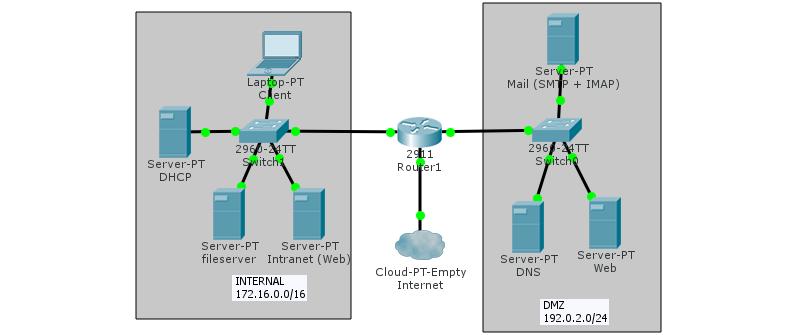
\includegraphics[width=\textwidth]{img/assignment-sme.png}
  \caption[Netwerkdiagram SME-opdracht]{Diagram van het op te zetten kantoornetwerk in de SME-opdracht. Links van de router bevindt zich het netwerk met publiek toegankelijke services (IP range 192.0.2.0/24), rechts het interne netwerk (172.16.0.0/16) met werkstations en netwerkservices voor intern gebruik. Merk op dat sommige van de vernoemde machines niet tot de opdracht behoren, maar enkel dienen als illustratie.}
  \label{fig:sme}
\end{figure}

Deze opdracht bestaat uit een aantal deeltaken:

\begin{itemize}
\item LAMP webserver
\item DNS server
\item Fileserver
\item DHCP server
\item Integratie, configuratie router
\end{itemize}

\subsection{High availability}
\label{subs:high-availability}

In de tweede opdracht verkennen we de taken van een \textit{site reliability engineer (SRE)}. Het is de bedoeling om de infrastructuur op te zetten voor een grote website die veel webtrafiek moet kunnen verwerken. Typisch worden de netwerkservices die samen de klassieke LAMP-stack vormen verdeeld over verschillende machines (zie Figuur~\ref{fig:ha}):

\begin{itemize}
\item Een \textit{load-balancer} verdeelt netwerktrafiek over \textit{verschillende webservers};
\item Een \textit{cache-systeem} zorgt dat niet alle requests leiden tot het opnieuw genereren van een pagina;
\item De \textit{database-backend} komt op een aparte server.
\end{itemize}

Bij dit soort opstellingen is het ook essentieel dat de beheerder een overzicht heeft van de correcte werking van alle componenten. Om dit te realiseren moet je een monitoring-systeem implementeren met een dashboard dat een overzicht geeft van het platform. Je moet in het bijzonder in staat zijn om de \textit{bottleneck resource} te identificeren, de hardware- of systeembron die het eerst verzadigd wordt door de binnenkomende trafiek. Dat kan de CPU zijn, het geheugen, I/O (netwerk of opslag), enz.

\begin{figure}
  \centering
  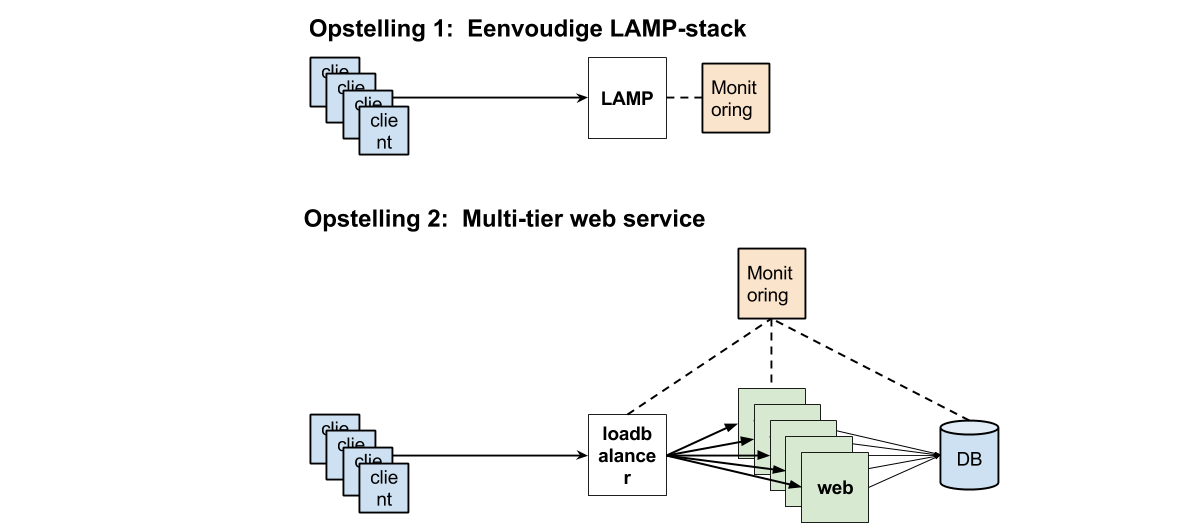
\includegraphics[width=\textwidth]{img/assignment-ha.png}
  \caption[Netwerkdiagram High Availability-opdracht]{Netwerkdiagram High Availability-opdracht. In een eerste opstelling draait de webserver in zijn geheel op een enkele VM met een monitoringsysteem voor de opvolging. Het einddoel is een opstelling waar alle services op aparte entiteiten draaien: een loadbalancer die requests verdeelt over een aantal webservers en een aparte database in de backend.}
  \label{fig:ha}
\end{figure}

\subsection{Continuous Integration/Continuous Delivery}
\label{subs:continuous-delivery}

Het derde jobprofiel dat je kan verkennen is dat van de \textit{release engineer}. Deze komt vooral voor in omgevingen waar webapplicaties de omzet van het bedrijf genereren, zoals bijvoorbeeld grote websites als Google, Amazon, Facebook, enz. De release engineer ondersteunt een team van software-ontwikkelaars om zo snel en zo vlot mogelijk nieuwe features in productie kunnen brengen. In plaats van grote, ingrijpende releases over langere periodes met veel nieuwe features, streeft men er tegenwoordig naar om kleinere releases te doen aan een hoger tempo (soms zelfs tientallen per dag), met bv.~slechts één nieuwe feature of verbetering. Voor deze manier van werken is specifieke infrastructuur nodig en is het nodig een aantal zaken verregaand te automatiseren.

De bedoeling van deze opdracht is om een Continuous Delivery ``build pipeline'' te bouwen voor een zelf te kiezen casus.

Typisch verloopt dat proces volgens deze stappen:

\begin{itemize}
\item De ontwikkelaar werkt op een ``development environment'' in de vorm van een virtuele machine aangestuurd door Vagrant
\item Wanneer de ontwikkelaar code publiceert op de ``master'' branch van een Git repository wordt het buildproces opgestart, bestaande uit:

  \begin{itemize}
  \item code-analyse, linting;
  \item compilatie (indien van toepassing);
  \item uitvoeren van unit tests;
  \item packaging (bv.~RPM, .deb, tarball);
  \item deployment in QA-omgeving (QA: Quality Assurance);
  \item uitvoeren van functionele tests;
  \item deployment in productie-omgeving.
  \end{itemize}

\item De ``QA environment'' is een VM op een zelf te kiezen virtualisatieplatform (bv. KVM, OpenNebula, Docker)
\item Wanneer alle tests slagen, wordt de nieuwe code automatisch gepromoveerd naar de volgende stap, in het beste geval tot en met de ``productie-omgeving'' op een cloud-platform (bv. Amazon AWS of DigitalOcean).
\end{itemize}

Je moet de hele pipeline kunnen demonstreren. Na een wijziging in de code te pushen moet je (na verloop van tijd) de wijziging op de productieserver kunnen zien.

De VMs die op de verschillende platformen draaien, worden toch zo identiek mogelijk geconfigureerd. Hier bestaan tools voor, bv.~Packer.  Je mag ook containers (bv. Docker) gebruiken om je applicatie in te pakken. De build server kan Jenkins zijn, je kan ook kijken naar Travis CI of Gitlab. Voor het laatste kan je gebruik maken van een abonnement op het Gitlab Gold Plan. Indien je hiermee wil werken, neem dan contact op met \href{mailto:bert.vanvreckem@hogent.be}{Bert Van Vreckem}.

Enkele concrete suggesties volgen hieronder. Behalve de Drupal-opdracht zijn dit allemaal reële casussen. Neem contact op met \href{mailto:bert.vanvreckem@hogent.be}{Bert Van Vreckem} indien je interesse hebt in deze opdrachten.

\begin{itemize}
  \item ASP.NET-applicatie op Docker\footnote{\url{https://www.docker.com/}}. Dit is een reële casus en het resultaat is in het beste geval een opstelling die in productie zal gebruikt worden binnen HOGENT. Recentelijk is er een nieuwe applicatie geschreven voor de administratieve opvolging van stages binnen de opleiding toegepaste informatica. Deze draait echter nog niet in productie. Jouw taak zou dan zijn om er voor te zorgen dat de applicatie kan worden gecompileerd en uitgerold in de productie-omgeving. De applicatie is geschreven om in Docker te draaien, dus via deze casus krijg je ook de kans daar ervaring mee op te doen. 
  
  \item Android application development. Dit is een reële casus en bestaat uit het verbeteren en stroomlijnen van een proof-of-concept van een Jenkins build-server voor het compileren van Android applicaties die op Google cloud draait.
  
  \item Geautomatiseerd testen van Ansible-rollen met Molecule\footnote{\url{https://github.com/ansible/molecule}}. Ook dit is een reële casus. De rollen \texttt{bertvv.bind}, \texttt{bertvv.vsftp}, enz. worden getest via Travis CI\footnote{Zie bijvoorbeeld \url{https://travis-ci.org/bertvv/ansible-role-bind}}. Voor elke ondersteunde Linux-distributie wordt een Docker-container opgestart waarop de Ansible-rol toegepast wordt, waarna er acceptatie-tests op uitgevoerd worden. Het testsysteem is ontwikkeld op een moment dat er nog geen algemeen gebruikte oplossingen bestonden voor het doorgedreven testen van Ansible-rollen. Het is gebaseerd op een shell-script en Docker images die specifiek voor deze toepassing zijn opgezet. Het onderhouden van de testinfrastructuur neemt veel tijd in beslag en regelmatig falen de tests omwille van fouten in het testsysteem. Molecule is een relatief nieuw systeem dat recent als het officiële Ansible-testplatform is verkozen. De bedoeling hier is om een proof-of-concept op te zetten voor het testen van de \texttt{bertvv.*}-rollen op basis van Molecule.
  
  \item Automatisch genereren van PDF-bestanden uit \LaTeX{}-broncode en publicatie op Github. De bedoeling is hier om vanuit een Github-repo met \LaTeX-{}be\-stan\-den bij elke push in Travis-CI een build-omgeving op te zetten, het bestand te compileren (incl.~bibliografie, index, enz.), en de resulterende PDF te publiceren op Github, onder Releases. Het systeem moet in staat zijn om bestanden met de HOGENT huisstijlsjablonen te compileren, waarvoor o.a. specifieke fonts nodig zijn (bv. Montserrat). In Travis-CI moet je alle nodige packages downloaden en installeren, wat veel tijd in beslag neemt. Een mogelijke benadering is vooraf een Docker-container te prepareren waar de compilatie in kan uitgevoerd worden\footnote{Bijvoorbeeld \url{https://github.com/Vincevrp/docker-tex}}. Die kan ook lokaal getest worden, wat tijd bespaart bij het troubleshooten.

  \item Ontwikkelen van Drupal plugins. De developer krijgt een VM met Drupal die toelaat om code te schrijven op het hostsysteem en die onmiddellijk zichtbaar is (bv. via VirtualBox shared Folders). Bij committen van code in het versiebeheersysteem worden linters/code analyzers uitgevoerd en geautomatiseerde tests. Eventueel kunnen tests op verschillende versies van PHP/MySQL/Drupal in parallel uitgevoerd worden. Als dit lukt, wordt een package gecreëerd dat kan gepubliceerd worden voor gebruikers.
\end{itemize}

\textbf{Opmerking.} Studenten die deze opdracht combineren met het DevOps-project wordt gevraagd om voor dit vak een andere casus te kiezen. Hetzelfde werk indienen voor twee verschillende vakken is een oneerlijk voordeel dat andere studenten niet hebben. Je kan wel voor beide vakken dezelfde achterliggende technologieën gebruiken zodat je de opgedane kennis wel in beide kan toepassen.

\section{Actualiteit}
\label{sec:actualiteit}

Bij elke rol in de ict-sector is het voortdurend bijwerken van je vakkennis onontbeerlijk om de snelle evolutie in je vakgebied bij te kunnen benen. In Linux systeembeheer is dat niet anders. Wat ons vakgebied kenmerkt is een uitgesproken wil om informatie en kennis te delen. \emph{Sharing is caring!} Er is dan ook een schat van informatie te vinden over de meest recente evoluties via blogs, conferenties waarvan de lezingen op Youtube of Vimeo gepubliceerd zijn, enz.

De bedoeling van deze taak is aan te tonen dat je deze evoluties ook opvolgt en probeert toe te passen in de praktijk. Je kan kiezen uit twee manieren om dit aan te tonen:

\begin{itemize}
  \item Pas een recentelijk gepubliceerde techniek, tool, \ldots{} toe op de opstelling van je hoofdopdracht;
  \item Doe een bijdrage aan een open source project gerelateerd aan de cursus (incl. tools en projecten die door de lector onderhouden worden\footnote{\url{https://github.com/bertvv/}}).
\end{itemize}

Samenwerken met één of enkele medestudenten is toegelaten. In dat geval moet elke student individueel kunnen aantonen een significante bijdrage geleverd te hebben via duidelijke rapportering, Git commits, \ldots

\textbf{Begin zo snel mogelijk hier aan te werken!} Wacht niet tot het einde van het semester om dan snel iets in elkaar te flansen. Dit kan leiden tot een beoordeling ``nog niet bekwaam,'' met als gevolg dat je niet kan slagen.

\subsection{Nieuwe technieken uitproberen}
\label{subs:nieuwe-technieken-uitproberen}

Zoals eerder aangegeven, vormen Linux-systeembeheerders een ``community'' waar er veel informatie uitgewisseld wordt. Sommigen gieten zaken die ze bijleren in een blog-artikel, gaan erover spreken op conferenties, enz.

De bedoeling hier is om zo'n artikel of lezing toe te passen op de labo-opdracht. Een paar voorbeelden als inspiratie:

\begin{itemize}
  \item \textcite{Hayden2015} en \textcite{Davila2015} beschrijven een manier om RHEL of CentOS-sys\-te\-men te testen op vlak van beveiliging, gebaseerd op Ansible. Is het mogelijk dat toe te passen op onze systemen? In het artikel gaat het over versie 6, terwijl wij op versie 7 zitten. In hoeverre kan dit aangepast worden?
  \item Gerelateerd aan het vorige voorstel: voer een security-audit uit met Lynis\footnote{\url{https://cisofy.com/lynis/}} op de VMs in je opstelling. Tracht de belangrijkste problemen op te lossen en verwerk dit in de Ansible-rollen die je gebruikt hebt. Dien eventueel een Pull Request in bij het Github-project van die rol.
  \item Fail2ban is een Intrusion Prevention System dat een server kan beschermen tegen brute-force of denial of service-aanvallen \autocite{Sawiyati2014}. Kan je dit toepassen op onze servers? Het is uiteraard wel de bedoeling dit via Ansible te doen. Dat kan hetzij via een bestaande rol (zie Ansible Galaxy), die je zo nodig aanpast, hetzij één die je zelf schrijft.
  \item Secure Shell is de standaard manier om Linux-servers op een veilige manier van over het netwerk te beheren. Maar volgens \textcite{stribika2015} is het mogelijk om \texttt{sshd} nog beter te beveiligen. Kan je dit toepassen op onze servers? Kan je eventueel een Ansible-rol voor het beher van \texttt{sshd} gebruiken en verbeteren op basis van het artikel?
  \item Zoals onze opstelling nu is, zullen wachtwoorden in de \texttt{host\_vars} of \texttt{group\_vars} bestanden opgeslagen worden. Dit is niet ideaal: we steken onze code in een versiebeheersysteem, maar wachtwoorden horen daar met het oog op beveiliging helemaal niet in thuis. Ansible heeft hiervoor een oplossing: Ansible Vault\footnote{\url{https://docs.ansible.com/ansible/playbooks_vault.html}}. \textcite{Blanc2015} beschrijft een methode om het gebruik van Ansible Vault zo transparant mogelijk te maken. Kan je het toepassen in onze opstelling?
  \item \textcite{Johnson2015} schreef een artikel over het versnellen van Ansible. Kloppen zijn aanbevelingen? Kan je dat aantonen, m.a.w. het tijdverschil meten tussen de standaardinstellingen en zijn aanpassingen?
\end{itemize}

Je kan de blogs waar naar gerefereerd werd in deze voorbeelden opvolgen (bv. via een RSS reader), hieronder volgen er nog enkele:

\begin{itemize}
\item AT Blog: \url{http://www.atcomputing.nl/blog/}
\item Cron Weekly newsletter: \url{https://www.cronweekly.com/}
\item Erika Heidi: \url{http://erikaheidi.com/blog/}
\item Everything Sysadmin (Tom Limoncelli): \url{http://everythingsysadmin.com/}
\item Everything is a Freaking DNS Problem (Kris Buytaert): \url{http://www.krisbuytaert.be/blog/}
\item Fedora Magazine: \url{http://fedoramagazine.org/}
\item Linux Action News: \url{https://linuxactionnews.com/}
\item Linux Journal: \url{http://www.linuxjournal.com/}
\item Major.io (Major Hayden): \url{https://major.io/}
\item ma.ttias.be (Mattias Geniar): \url{https://ma.ttias.be/}
\item Planet CentOS: \url{http://planet.centos.org/}
\item Runaway Sequence (Aaron Hunter): \url{http://sharknet.us/}
\item Standalone Sysadmin (Matt Simmons): \url{https://www.standalone-sysadmin.com/blog/}
\item SysadminCasts (Justin Weissig): \url{https://sysadmincasts.com/}
\item The Geek Stuff: \url{http://www.thegeekstuff.com/}
\end{itemize}

Vond je andere interessante blogs? Geef maar door aan de lectoren! Andere bronnen van informatie zijn Youtube of Vimeo (voor presentaties van conferenties of screencasts), Twitter, enz.

Ben je zelf buiten de opleiding om bezig met Linux? Bespreek met de lector of je je ervaringen, experimenten, \ldots{} eventueel kan inbrengen voor deze opdracht.

\subsection{Bijdrage aan een open source project}
\label{subs:bijdrage-aan-een-open-source-project}

Alle tools waar we in de cursus gebruiken zijn open source. Sommige, zoals Ansible, werden door een softwarebedrijf ontwikkeld die daar een businessmodel rond gebouwd hebben. Andere werden door enthousiastelingen in hun vrije tijd ontwikkeld. In elk geval kunnen we gratis gebruik maken van software van hoge kwaliteit, dankzij de inspanningen van velen.

Het is passend daar iets voor terug te doen, dus de bedoeling is om een significante bijdrage te leveren aan een open source project dat gerelateerd is aan de cursus. Dit kan een kleine bijdrage zijn, maar voorwaarde is wel dat ze aanvaard is door de auteur(s) van het project.

Je mag hiervoor samenwerken met één of meerdere medestudenten, maar de individuele bijdrage van elk teamlid moet aantoonbaar zijn (bv. aan de hand van Git commits). Zet hiervoor een aparte, publieke Github repository op, en verwijs er naar vanuit je laboverslag voor deze opdracht.

Enkele mogelijkheden:

\begin{itemize}
  \item Op Ansible Galaxy zijn veel rollen te vinden die beter kunnen, of waar de auteur niet genoeg tijd heeft om zaken toe te voegen of fouten op te lossen. Implementeer een nieuwe feature, zorg er voor dat ze op CentOS 7 draaien, verbeter fouten, \ldots{} Ook de lector apprecieert hulp bij het verder ontwikkelen van zijn Ansible-rollen \url{https://galaxy.ansible.com/bertvv/} en \url{https://github.com/search?q=user\%3Abertvv+ansible}.

  Het resultaat wordt ingediend als een Pull Request, de code volgt de richtlijnen voor stijl\footnote{\url{https://github.com/bertvv/ansible-role-skeleton/wiki}}, en wordt getest. Opties zijn niet \emph{hard-coded} maar blijven instelbaar via rolvariabelen. Waar mogelijk wordt een standaardwaarde gekozen die in de meeste gevallen het beste resultaat geeft, of wordt aan de hand van de eigenschappen van het systeem een waarde ``berekend'' of bepaald die voor dat systeem optimaal is. Alle nieuwe variabelen/features worden goed gedocumenteerd.
  
  Voor concrete ideeën kan je de Issues bekijken op het Github-project en één ervan op je te nemen.

  \item Schrijf een Ansible rol (waar nog geen alternatief voor CentOS voor bestaat) en publiceer die op Ansible Galaxy. Dit doe je best in samenwerking met één of meerdere medestudent(en)! Wanneer je voor de hoofdopdracht een nieuwe Ansible rol schrijft, kan je die algemeen bruikbaar maken en publiceren.
  
  \item Pas een techniek die beschreven is voor een andere distributie (CentOS 6, Debian, Ubuntu, \ldots{}) toe op CentOS 7. In de vorige sectie vind je een paar concrete voorbeelden.
\end{itemize}

Andere ideeën zijn ook welkom, bespreek die met de lector. Ook op Chamilo kan je nog enkele voorstellen vinden.

\section{Rapportering en documentatie}
\label{sec:rapportering-en-documentatie}

In de \texttt{assignment/} directory van je repository komt alle documentatie terecht in verband met de labo-taken. Het gebruikte formaat is Markdown~\autocite{Gruber2004,Github2016}, wat de standaard geworden is voor documentatie op Github (en ook andere Git hosting-oplossingen zoals Gitlab of Bitbucket). Markdown is een eenvoudig tekstformaat dat kan gerenderd worden als HTML, of makkelijk naar andere formaten kan omgezet worden (PDF, \LaTeX\, presentatie met reveal.js, enz.). Leer het formaat goed kennen en controleer of je verslagen duidelijk leesbaar zijn (op Github of reeds lokaal met een editor met Markdown-ondersteuning). Gebruik bv. codeblokken met syntax colouring, links naar relevante code elders in de repository, enz.

\subsection{Laboverslagen}
\label{subs:laboverslagen}

Er is een sjabloon voorzien voor de laboverslagen. Pas dit sjabloon aan voor jezelf, vul bovenaan je naam in. Voor elke deeltaak maak je een apart verslag, waar je in detail uitlegt wat je precies gedaan hebt. Hoe heb je de taak aangepakt? Welke bronnen heb je gebruikt? Reflecteer ook over je vooruitgang: wat ging goed/niet goed? Wat heb je geleerd? Waar zit je vast, waar heb je nog problemen mee? Let wel: het is niet de bedoeling om code te gaan knippen en plakken in je laboverslag!

Bij elk laboverslag hoort een testplan en -rapport. Het testplan is een opsomming van alle handelingen die nodig zijn om aan te tonen dat het op te zetten systeem zich gedraagt volgens de specificaties.

Het testplan is eigenlijk het scenario van de demo die je geeft aan de lector om aan te tonen dat je alle aspecten van de opdracht correct hebt uitgevoerd. Dit bestaat uit concrete handelingen of commando's die je moet uitvoeren, en een beschrijving van het verwachte resultaat.

Door het lezen van het testrapport moet het duidelijk zijn in hoeverre de opdracht is uitgevoerd, wat het effectieve resultaat van de tests was. Je kan transcripties toevoegen van de terminal (gebruik hiervoor Markdown codeblokken, geen screenshots!). Het testrapport zou evenveel informatie moeten bevatten als de demo.

Ook bij de \textbf{troubleshooting-oefeningen} hoort een verslag. Deel je verslag op in secties voor de verschillende fasen in het troubleshooting-proces. Je kan je verslag al voorbereiden door de commando's die je zeker moet uitvoeren er alvast in op te sommen, samen met verwachte resultaten (voor zover dit al op voorhand kan). Sla dit op als een apart sjabloon specifiek voor troubleshooting. Bij het uitvoeren van de oefening kan je dit dan aanvullen met de effectieve resultaten die je krijgt, en de commando's/configuratiewijzigingen die je hebt uitgevoerd om problemen op te lossen.

\subsection{Cheat-sheets en checklists}
\label{subs:cheat-sheets-en-checklists}

Wanneer je niet gewend bent om met Linux te werken, dan is het niet evident om op te zoeken en te onthouden welke commando's je nodig hebt voor welke taak. Via Google vind je wel vaak een oplossing, maar dat ligt niet altijd voor de hand. Er zijn bijvoorbeeld recentelijk substantiële wijzigingen doorgevoerd in de architectuur van de belangrijkste Linux-distributies waardoor bepaalde commando's (die je erg vaak tegenkomt bij Googlen) niet meer werken.

Om jezelf te helpen bij het onthouden van de belangrijkste commando's, is het bijhouden van een cheat-sheet of ``spiekbriefje'' een nuttig hulpmiddel. Als je een bepaald commando een paar keer bent moeten gaan opzoeken, dan is het best dat eens te noteren zodat je het in de toekomst sneller terugvindt en op de duur ook beter onthoudt.

Hetzelfde geldt voor procedures van handelingen die steeds terugkomen.  Bijvoorbeeld, als je wil nagaan of de IP-instellingen van een host kloppen, gebruik je altijd dezelfde commando's. Wanneer je die telkens opnieuw moet gaan opzoeken verspil je tijd en het is best mogelijk dat je zo zaken over het hoofd ziet. Door checklists bij te houden, verminder je het opzoekwerk en kan je ook vlotter werken~\autocite{Simmons2009}.

Je kan inspiratie opdoen op deze Github-repository waar een aantal cheat-sheets en checklists gepubliceerd zijn: \url{https://github.com/bertvv/cheat-sheets}.

Bij de evaluatie wordt er rekening mee gehouden hoe je deze documenten hebt bijgehouden in de loop van het jaar (aan de hand van de commit log).

\subsection{Bloggen}
\label{subs:bloggen}

Technische blogs zoals deze die eerder aangehaald werden zijn een meer en meer voorkomende manier om ervaringen en informatie uit te wisselen binnen ons vakgebied. Studenten die gaan solliciteren (en ook wie al in het vak staat) kunnen met een eigen blog aan potentiële werkgevers aantonen dat ze gepassioneerd zijn door hun vak, bezig zijn met de laatste technologieën en open staan voor het delen van kennis. Je kan een eigen blog opstarten en schrijven over wat je in deze cursus (en ook andere!) leert, zaken die je zelf opgezocht en ondervonden hebt, \ldots

Voorbeeldjes:

\begin{itemize}
\item Jürgen Van Meerhaeghe: \url{https://jurgenvm.blogspot.be/}
\item Stijn Spanhove: \url{http://www.spanhove.com/blog.htm}
\item Thomas Clauwaert: \url{https://ciberth.blogspot.be/}
\item Toon Lamberigts en Tomas Vercautter: \url{https://t0t0.github.io/}
\end{itemize}

Dit is vrijblijvend, maar heeft wel een positieve invloed op je examencijfer.




%---------- Back matter -------------------------------------------------------
% In de bibliografie niet de bronnen uit voorbeeld.bib afdrukken. Alle bronnen
% in voorbeeld.bib moeten in het veld ``keywords'' ook de term ``voorbeeld''
% bevatten.
\printbibliography[notkeyword=voorbeeld]
\addcontentsline{toc}{chapter}{\textcolor{maincolor}{\IfLanguageName{dutch}{Bibliografie}{Bibliography}}}

\end{document}

